% !TEX root = main.tex

\section{はじめに}

ムーアの法則が限界を迎え,CPUのコア単位の性能向上はほとんど止まっている.
現在のコンピュータ技術ではCPUに搭載された複数のコアを活用するマルチスレッド処理が主流となっており,マルチスレッドを効果的に使用するソフトウェアやデータ構造などが提案されている.
索引技術においてもその傾向は同様であり,近年ではメニーコアCPU上でのマルチスレッド処理を意識した索引構造が多く提案されている.

代表的な索引構造である\Bptree{}~\cite{book:dbsystem}では,ロックを用いた同時実行制御が行われている.
しかし,マルチスレッド処理においてロックによる同時実行制御は多数の待ちスレッドが発生するため,スケーラビリティが悪化する.
そこで,\Bptree{}を基に構造変更時のロックの占有期間を短くした\Blinktree{}~\cite{tods1981:Lehman}や,楽観的な制御を用いることで\Blinktree{}における読み取り時のロック取得を不要にしたOLFIT~\cite{vldb2001:Cha}などがある.
更に,読み取りおよび書き込みの両方においてロックを取得しないロックフリー索引としてBw木~\cite{book:Bwtree}およびBz木~\cite{book:Bztree}が提案されている.
しかし,これらのロックフリー索引は書き込みの際に競合や多数のスレッドの失敗が発生することによって,マルチスレッド環境では性能が向上していない.
そのため,ロックフリー索引には改善の余地が残されていると考えられる.

本研究では\Bptree{}の同時実行制御においてロックフリーアルゴリズムを活用した,新たな索引構造である同時実行\Bptree{}(concurrent B$^{+}$-tree, \Bctree{})を提案する.
特に,本論文ではその構造および操作について述べる.

本稿の構成は以下の通りである.
\Sec{\ref{sec:relatedwork}}では,関連研究としてロックの取得期間の短縮を狙った索引やロックフリー索引などについて概説する.
次に,\Sec{\ref{sec:bc_tree_structure}}で\Bctree{}の構造について説明し,\Sec{\ref{sec:node_operation}}および\Sec{\ref{sec:smo}}で\Bctree{}の操作について述べる.
なお,本稿では削除およびマージ操作については議論しない.
最後に,\Sec{\ref{sec:conclusion}}で本稿のまとめと今後の方針を述べる.

\section{関連研究}
\label{sec:relatedwork}

近年では,ロックを取得しないロックフリー索引に対して注目が集まっている.
本節では関連研究として,ロック期間の短縮を狙った索引である\Blinktree{}と楽観的制御により読み取り時のロック取得を不要にしたOLFIT,そして代表的なロックフリー索引であるBw木およびBz木について説明する.

\subsection{\Blinktree{}}

\Blinktree{}~\cite{tods1981:Lehman}は,\Bptree{}の各ノードが右兄弟へのリンクを持った構造をしている.
リンクを持つことにより,親ノードからさかのぼらずに隣接するノードに達することができる.
また,\Blinktree{}はノード内にハイキーを持つことにより,並行する構造変更操作にも対応できる.
例えば,構造変更後の新たなノードが兄弟ノードからリンクによって参照されているが,親ノードからの子ポインタによって参照されていない場合がある.
この時に同時に検索操作が起きていた場合,たどり着いたノードのハイキーよりも検索キーが大きければ,構造変更操作が並行して起きたとして兄弟リンクをたどり正しいノードにたどり着くことができる.
兄弟リンクとハイキーを持つことにより,ロックを取るノードを最小限に抑え,単一操作内でのロック期間を短縮している.

\subsection{OLFIT}

OLFIT~\cite{vldb2001:Cha}は,\Blinktree{}においてバージョン番号を採用することにより,ノードの更新を管理し楽観的制御を実現している.
書き込み操作は\Blinktree{}と同様にロックを用いて動作する.
一方読み取り操作では,ノードをロックしない代わりにバージョン番号を読み取っておく.
検索対象を読み取った後,バージョン番号が読み取り前と同じか検証する.
バージョン番号が変化していなければ読み取った値を返し,変化している場合には再度読み取り操作を始めからやり直す.

\subsection{Bw木}

Bw木~\cite{book:Bwtree}は,直感的にはロックフリーの単方向連結リストと\Bptree{}を組み合わせた索引構造である.
Bw木は追記型の差分レコードとマッピングテーブルを採用している.
ノードの更新を一括に処理し,単一のCAS命令を用いてノード間のポインタをインストールできるようメモリ内のデータ構造を設計することにより,木のロックフリー化を実現している~\cite{book:DatabaseInternals}.

更新内容が記述された差分レコード(delta record)をノードの前に連結リストとして挿入し,索引に対する全ての更新を表す.
差分レコードのリストが一定以上の長さを持つとき,ノードの統合操作が行われ,統合後は\Bptree{}のノードと同様のものが生成される.

マッピングテーブルはノード間のリンクを仮想化し,メインメモリ上の差分更新を可能とする.
各ノードは自身の子ノードや兄弟ノードへのポインタを直接持つ代わりにマッピングテーブル上のID(logical page ID, LPID)を持つ.
つまり,マッピングテーブルを用いてLPIDを実際のポインタへと変換することでノードを辿る.

\subsection{Bz木}

Bz木~\cite{book:Bztree}は,\Bptree{}の葉ノード内部にロックフリーの固定長配列を持つ索引構造である.
Bz木は,Bz木の根を示すルートポインタと,複数の内部ノードと葉ノードからなる.
ルートポインタが木の根となるノードへのポインタを持ち,根ノードおよび中間ノードなどの内部ノードが子となる内部ノードまたは葉ノードへのポインタを持つ.
Bz木は単一のCAS命令ではなく,メモリ上の複数のワードを対象とするmulti-word compare-and-swap(MwCAS)命令を用いて木のロックフリー化を実現している.

Bz木の各ノードにはヘッダ,メタデータ,レコードが格納されている.
ヘッダにはステータスワードというフィールドが格納されており,ステータスワードはCAS命令や構造変更操作の制御,ノード内のレコード数などノード更新時に必要な情報を格納している.
Bz木はノードに対する書き込みおよび構造変更操作をステータスワードを更新することによってロックフリーに実現している.

\section{\Bctree{}の構造}
\label{sec:bc_tree_structure}

% Bc木の概要
\Bctree{}はBw木とBz木の構造を参考に,各構造の長所を組み合わせた索引構造である.
\Bctree{}の概形を\Fig{\ref{fig:bc_tree-structure}}に示す.
木の論理的な構造は\Blinktree{}に則っており,各ノードが同じ階層の右兄弟への参照リンクを持つ.
各ノードへの参照はマッピングテーブルを用いた間接参照を採用し,マッピングテーブル内の物理ポインタを差し替えることでそのノードへの参照を一括で変更する.

\begin{figure*}[t]
    \centering
    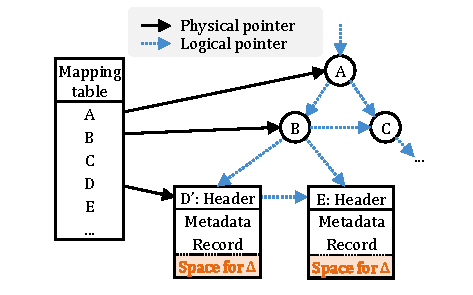
\includegraphics{./figures/Bc-structure.pdf}
    \caption{\Bctree{}の概形}
    \label{fig:bc_tree-structure}
\end{figure*}

% Bc木ノードの説明
\Bptree{}と同様に,\Bctree{}は索引層およびデータ層によって構成される.
索引層のノード(中間ノード)は分割キーと子ノードへのポインタの組を格納し,木の下方への検索を補助する.

各ノードの領域はイミュータブル領域とミュータブル領域に分けられる.
イミュータブル領域はノードヘッダおよびソート済みのレコードを格納する.
ヘッダはイミュータブル領域の情報を管理し,構造変更時のみその値が変更される.
ミュータブル領域はステータスワードの格納と差分レコードを挿入するための書き込みバッファの役割を果たす.
ステータスワードはミュータブル領域の情報を管理し,ノードの現在の状態や残容量などを管理する.
各ノードへ構造変更操作を行う際は,構造変更後のノードから構造変更前のノードへ物理リンクを張り,古いノードへの参照を可能にする.
なお,古いノードは構造変更が済み次第,ガベージコレクションへ追加され,他のスレッドから参照されないことが保証された時点で削除される.

% Bw木の欠点の克服
\Bctree{}はBw木およびBz木でそれぞれボトルネックとなる箇所を以下の通りに克服している.
Bw木では差分レコードによって更新を実現しているが,差分レコードは各スレッドによって独立にそのメモリ領域が確保されるため,同じノード上の差分レコードであってもメモリ上の配置は連続とならない.
そのため,差分レコードの探索はランダムアクセスとなり,キャッシュヒット率が低くなる.
そこでBz木で用いられたノード内書き込みバッファを採用することで,Bw木で発生していた差分レコードによるキャッシュミスを削減している.

% Bz木の欠点の克服
一方で,Bz木の差分レコードの挿入手続きにも改善の余地がある.
Bz木は差分レコードの書き込み時に,まずMwCAS命令を用いたステータスワードの更新によって差分レコード用の領域を予約する.
その後差分レコードを書き込み,メタデータをMwCAS命令により更新することで差分レコードを可視化する.
このとき,ステータスワードもMwCAS命令の対象とすることで同時に発生した構造変更操作を検知し,必要に応じて書き込み命令をアボートおよびリトライする.
しかしこのような手続きはステータスワードを不要に更新してしまい,スレッド間の競合を増加させてしまう.
そこで,\Bctree{}では同時に発生した書き込み命令と構造変更操作に対し,書き込み命令を優先するという方針を取る.
これにより,差分レコード可視化におけるステータスワードの確認が不要となり,書き込み命令におけるスレッド間の直接的な競合は領域予約のためのステータスワードの更新のみに抑えられる.

\section{\Bctree{}のノード操作}
\label{sec:node_operation}

本節では,\Bctree{}のノード操作について述べる.
\Bctree{}は以下の読み取りおよび書き込み操作をサポートする.

\subsection{書き込み}

% 書き込み操作の概要
書き込み操作はキーとペイロードを差分レコード領域に挿入する操作である.
キーが属する書き込み先の葉ノードを根ノードから二分探索により特定する.
挿入先の葉ノードに到達後,その葉ノードの差分レコード領域に値を挿入する.

% 書き込み操作の具体的な手順
書き込み操作は差分レコード領域の予約とレコード挿入および可視化の2ステップで行われる.
\Fig{\ref{fig:bc_tree_insertion}}に\Bctree{}における差分レコードの挿入を示す.
ノードフッタにはミュータブル領域の状態を表すステータスワードを用意し,この中のレコード数と使用済みブロックサイズを加算することで差分レコード用の領域を予約する.
また,\Bctree{}ではノードの生成時にミュータブル領域をゼロ埋めしている.
\Bctree{}では,メタデータがゼロ埋めされている場合を処理途中として表すため,差分レコード用の領域を予約した時点ではレコードが可視化されていないことを認識できる.
確保した領域へ差分レコードを書き込み,対応するレコードメタデータの値を更新することでレコードを可視化し,挿入処理を完了する.

\begin{figure}[t]
    \centering
    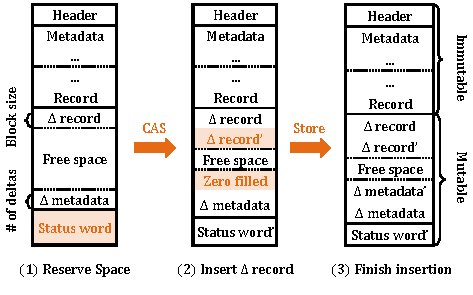
\includegraphics{./figures/Bc-insertion.pdf}
    \caption{\Bctree{}における差分レコードの挿入}
    \label{fig:bc_tree_insertion}
\end{figure}

% 書き込みができない場合の対処
以上の書き込み操作によって差分レコードを挿入していくが,挿入後の差分レコードの総数またはノード容量のしきい値を越える場合,差分レコードの統合操作または構造変更操作が行われる.
しきい値の確認はステータスワードの更新時に行われ,しきい値を越えた場合はレコードの書き込み後に統合操作,構造変更操作いずれかの操作を行うか判定する.

% Bc木の書き込み操作の特徴
書き込み処理はロックフリーに動作する.
書き込み同士の競合はステータスワードで解決され,差分レコード用領域の予約,つまり差分レコードの書き込み順はCAS命令の成功順によって順序付けられる.
また,後述する構造変更操作との競合によって待ち時間が発生しうる.

\subsection{読み取り}

% 読み取り操作の概要とミュータブル領域での読み取り
読み取り(Read)は与えられた対象キーのペイロードを返す操作である.
対象キーが与えられたとき,根ノードからの二分探索によりキーが属する葉ノードに到達する.
葉ノードに到達した後は,葉ノード内の差分レコードの線形探索とイミュータブルレコードの二分探索の2ステップで読み取り操作を行う.
最新の値は差分レコード領域に書き込まれるため,まずミュータブル領域を線形探索し,一致するキーがあるか確認する.
このとき,差分レコードの数はステータスワードから読み取り,差分レコードが可視化されていなければスキップする.

% ミュータブル領域にレコードがない場合
差分レコード中に対象のレコードが存在しなければ,ノードヘッダからイミュータブルレコードの数を読み取り,二分探索によって対象キーの有無を確認する.
先頭ノードが統合操作の途中である場合には,差分レコードを読み終わった時点で物理ポインタをたどり古いノードへ移動し,同様の2ステップを古いノード上で行う.

% Bc木における読み取り操作の特徴
読み取り処理はwait-freeに動作する.
上述したとおり読み取り命令は一切ノードの状態を変更せず,読み取った状態に応じて適切な手続きを選択する.
そのため,読み取り命令においてリトライなどは発生せず,有限時間内で必ず処理が終了する.

\section{\Bctree{}の構造変更操作}
\label{sec:smo}

\Bctree{}は構造変更操作として差分レコードのノードへの統合およびノードの分割操作を持つ.
構造変更操作を始める前に,新たなノードをマッピングテーブルに挿入することで,他のスレッドの待ち時間を削減する.

\subsection{統合}

% 統合操作の概要
統合操作は差分レコードの数またはノードの容量がそれぞれのしきい値を越えた場合,差分レコードとイミュータブルレコードをソートしてイミュータブル領域に反映する操作である.
統合操作を行うことで,ミュータブル領域を確保し新たな差分レコードの挿入を受け付ける.

% 統合操作の具体的な手順
\Fig{\ref{fig:bc_tree_consolidastion}}に\Bctree{}における統合操作を示す.
統合が必要になった場合,新たなノード領域を用意する.
そして,古いノードのステータスワードを更新後,ノードヘッダの情報から統合後に必要なイミュータブル領域を計算する.
なお,このステータスワードの更新により古いノードは全体がイミュータブルとなり,新たな差分レコードは挿入できなくなる.
次に,新たなノードにおいてステータスワードを含むヘッダ情報のみを更新した後,新規ノードとしてマッピングテーブル上の参照を更新する.
その後,古いノード上の差分レコードをイミュータブルレコードへ反映させつつ,新たなノードへレコードをコピーする.
最後に,統合後の状態でノードヘッダを更新し,新しいノードにおけるイミュータブル領域を可視化する.
この際に,後述する分割操作で用いられる分割キーを,統合後のノードのイミュータブル領域から計算する.

\begin{figure}[t]
    \centering
    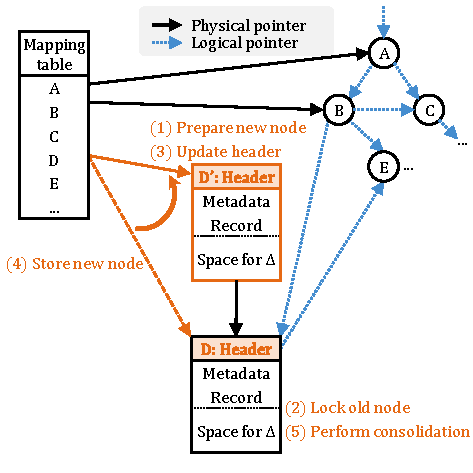
\includegraphics{./figures/Bc-consolidate.pdf}
    \caption{\Bctree{}における統合操作}
    \label{fig:bc_tree_consolidastion}
\end{figure}

% 統合操作時の書き込みについて
統合操作を行っている際に,発生した書き込み操作は新規ノードのミュータブル領域で受け付ける.
これにより統合操作の間も,読み取り操作は新規レコードのミュータブル領域,統合前のノードのミュータブル領域およびイミュータブル領域の順でレコードを確認することで読み取り操作を実行できる.

\subsection{分割}

% 分割操作の概要
分割操作はノードの差分レコードの数またはノード容量がそれぞれしきい値を越えており,統合後も十分なミュータブル領域を確保できない場合に,そのノードのレコードを新規の2つのノードに分散させる操作である.
分割操作により,容量が一杯になったノードを2つに分け,新たな差分レコードの挿入を受け付ける.

% 分割操作の具体的な手順
\Fig{\ref{fig:bc_tree_split}}に\Bctree{}における分割操作を示す.
構造変更操作が必要になった場合,新たなノード領域を2つ用意する.
ステータスワードの更新により対象ノード全体をイミュータブル状態にした後,レコードコピーを始める前に用意したノードをマッピングテーブルに挿入する.
これを実現するために,各ノードは自身の分割キーの位置を統合および分割操作のたびに記録する.
分割したノードの挿入後,統合操作と同様の手続きでレコードをコピーする.
分割時には,古いノードの分割キー未満の全てのレコードを左ノードにコピーする.
残りのレコード,すなわち分割キー以上の全てのレコードは右ノードにコピーする.

\begin{figure*}[t]
    \centering
    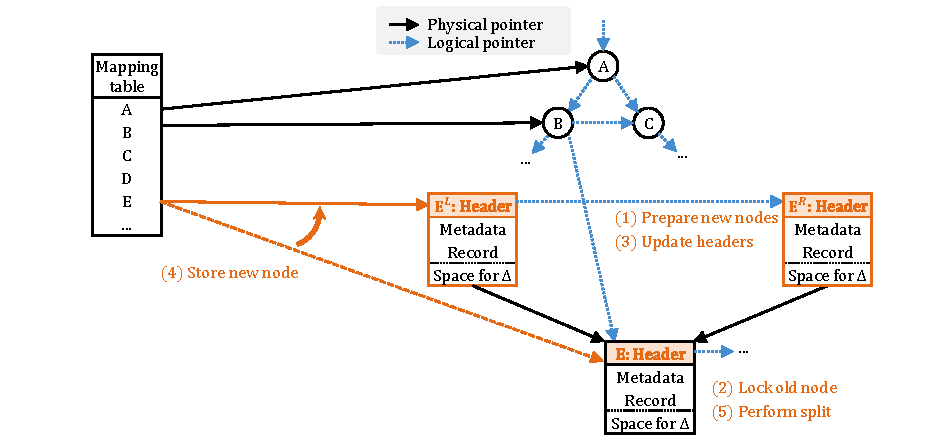
\includegraphics{./figures/Bc-split.pdf}
    \caption{\Bctree{}における分割操作}
    \label{fig:bc_tree_split}
\end{figure*}

% 右子ノードのリンクの反映の遅延
レコードのコピー後は,親ノードに右分割ノードへのリンクを挿入することで分割操作が完了する.
このとき,親ノードへはリンクの情報のみを挿入し,反映は親ノードの統合操作時に行う.
例えば新規ノードEを挿入した際,\Fig{\ref{fig:bc_tree_inner_nodes}}に示すように差分レコード領域に子ノードへのリンク情報のみを追記し統合操作が行われるまでそのリンクの反映を遅延する.
つまり,索引の探索中において中間ノードでは差分レコードを確認せず,イミュータブル領域のレコードのみを検索する.

% リンクの反映の遅延の理由
これは中間ノードにおけるCPUキャッシュ効率を高めることを狙っている.
親ノードのデータがCPUキャッシュ上に存在しており,ノードヘッダが同一のキャッシュラインに収まっていると想定する.
この時,左の子ノードの兄弟リンクを経由して右の子ノードに達するために必要な同期はノードヘッダおよびキー範囲の確認の2回のみである.
一方,右の子ノードへのリンクを挿入しかつそれを利用する場合,ノードヘッダ,メタデータおよびレコードの最低3回の同期が必要となる.
親ノードから子ノードへのリンクを有効的に利用できるのはその子ノードを対象とした操作のみであることを考えると,親ノードに右の子ノードへのリンクを即座に反映した手法ではキャッシュ効率が悪化してしまう.
そこで親ノードへはリンクの情報のみを挿入し,親ノードの統合操作時にリンクを反映させることによって,中間ノードにおけるCPUキャッシュの利用効率を高める.
更に,中間ノードのデータ量は葉ノードに比べて小さく変更も少ないため,CPUキャッシュは特に索引層において効率的に使用される.
よって,中間ノードでは基本的にイミュータブル領域のみを参照させることで読み書き両方において葉ノード探索の効率を向上できる.

\begin{figure}[t]
    \centering
    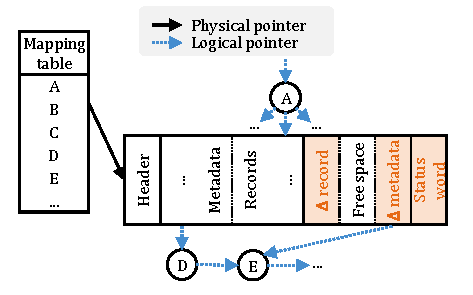
\includegraphics{./figures/Bc-inner_nodes.pdf}
    \caption{\Bctree{}における新規ノードEの挿入に伴う変更箇所}
    \label{fig:bc_tree_inner_nodes}
\end{figure}

\subsubsection{分割時の偏りの抑制}

% 分割キーについての注意
分割キーはイミュータブルレコードから決定される.
つまり差分レコードは考慮されないため,分割操作時に片方のノードにレコードの偏りが発生しうる.
前述した通り,分割操作前にノードを用意するため,イミュータブル領域および対応するメタデータ数は余裕を持って確保しておく必要がある.
そのため,差分レコードが片方のノードに集中し,その分のスペースがもう片方のノードで使用されない,未使用なイミュータブル領域が残る可能性がある.

% ノードの偏りへの対応
このような問題に対する対応策として,分割後の左右両ノードが一定以上の容量を持つようにすることが挙げられる.
分割後の左右両ノードが一定以上の容量を持つ場合には分割操作を行い,持たない場合には統合操作を行うようにする.
統合操作によって分割キーの位置が変化するため,書き込みの偏りが起きた場合においても,差分レコードが片方のノードに集中する事態をある程度防ぐことができる.
このような対応により,未使用になるイミュータブル領域を削減し,メモリを効率的に利用できる.

\subsubsection{Hotノードの検出および分割}

% 書き込みの偏りによる構造変更操作の競合について
\Bctree{}では,構造変更操作中のノードに対する書き込み操作が偏っている場合,次の構造変更操作が要求され構造変更操作同士が競合する可能性がある.
その場合の対応策について述べる.

% 書き込みの偏りによる問題
\Bctree{}では統合および分割による新規ノードの配置後,新規のノードは古いノードからのレコードコピーをしつつ,差分レコードの挿入を受け付ける.
その際書き込みの偏りが大きい場合,イミュータブル領域を可視化する前,つまり自身の構造変更操作が完了する前に次の構造変更操作が要求されてしまう.
索引においてレコードアクセスには偏りが発生しやすく,書き込みによって偏りが発生すると構造変更操作の競合などにより性能が劇的に低下する.
\Bctree{}ではそのような書き込みの集中したノードをHotノードと呼ぶ.

% 書き込みの偏りに対する対応
書き込みの偏りによる構造変更操作の競合に対して,先に行われた構造変更操作の完了後,分割操作を行う.
これにより,アクセスが偏っているレコード群を細かく分割し競合を緩和させ,かつ差分レコードを書き込むための領域を広く確保できるようになる.
このようなノードの積極的な分割によりレコードアクセスが偏るようなワークロードに対しても安定した性能を達成できる.

\section{おわりに}
\label{sec:conclusion}

本稿では\Bptree{}の同時実行制御においてロックフリーアルゴリズムを活用した,新たな索引構造である\Bctree{}について提案し,その構造および操作を紹介した.
今後は提案した索引構造を実装し,ノードのレコードを他のノードとつなぎ合わせるようなマージ操作など,他の操作を実装する.
また,代表的な索引構造である\Bptree{}や,近年提案されているBw木やBz木といったロックフリー索引との性能を比較検証する.